\def\QRCODE{MASTER_mispa_TUT.IMG.wavelets_matlabqrcode.png}
\def\QRPAGE{http://www.iptutorials.science/tree/master/MASTER_mispa/TUT.IMG.wavelets/matlab}
\mcorrectionsection{Matlab correction}

% \begin{tikzpicture}[remember picture,overlay]
%   \fill[orange] 
%   (current page header area.north west) 
%     rectangle
%   ([xshift=100pt,yshift=0pt]current page.east|-current page header area.south east);
% \end{tikzpicture}


\begin{note}This correction illustrates the wavelet decomposition in 1D or 2D.\end{note}

\subsection{1D signals}
Two functions are required: a function that loops over the different scales and calls the second function that performs the single step wavelet decomposition. The Haar wavelet is illustrated in Fig.\ref{fig:wavelets:matlab:haar}.

\begin{figure}[htbp]
 \centering
 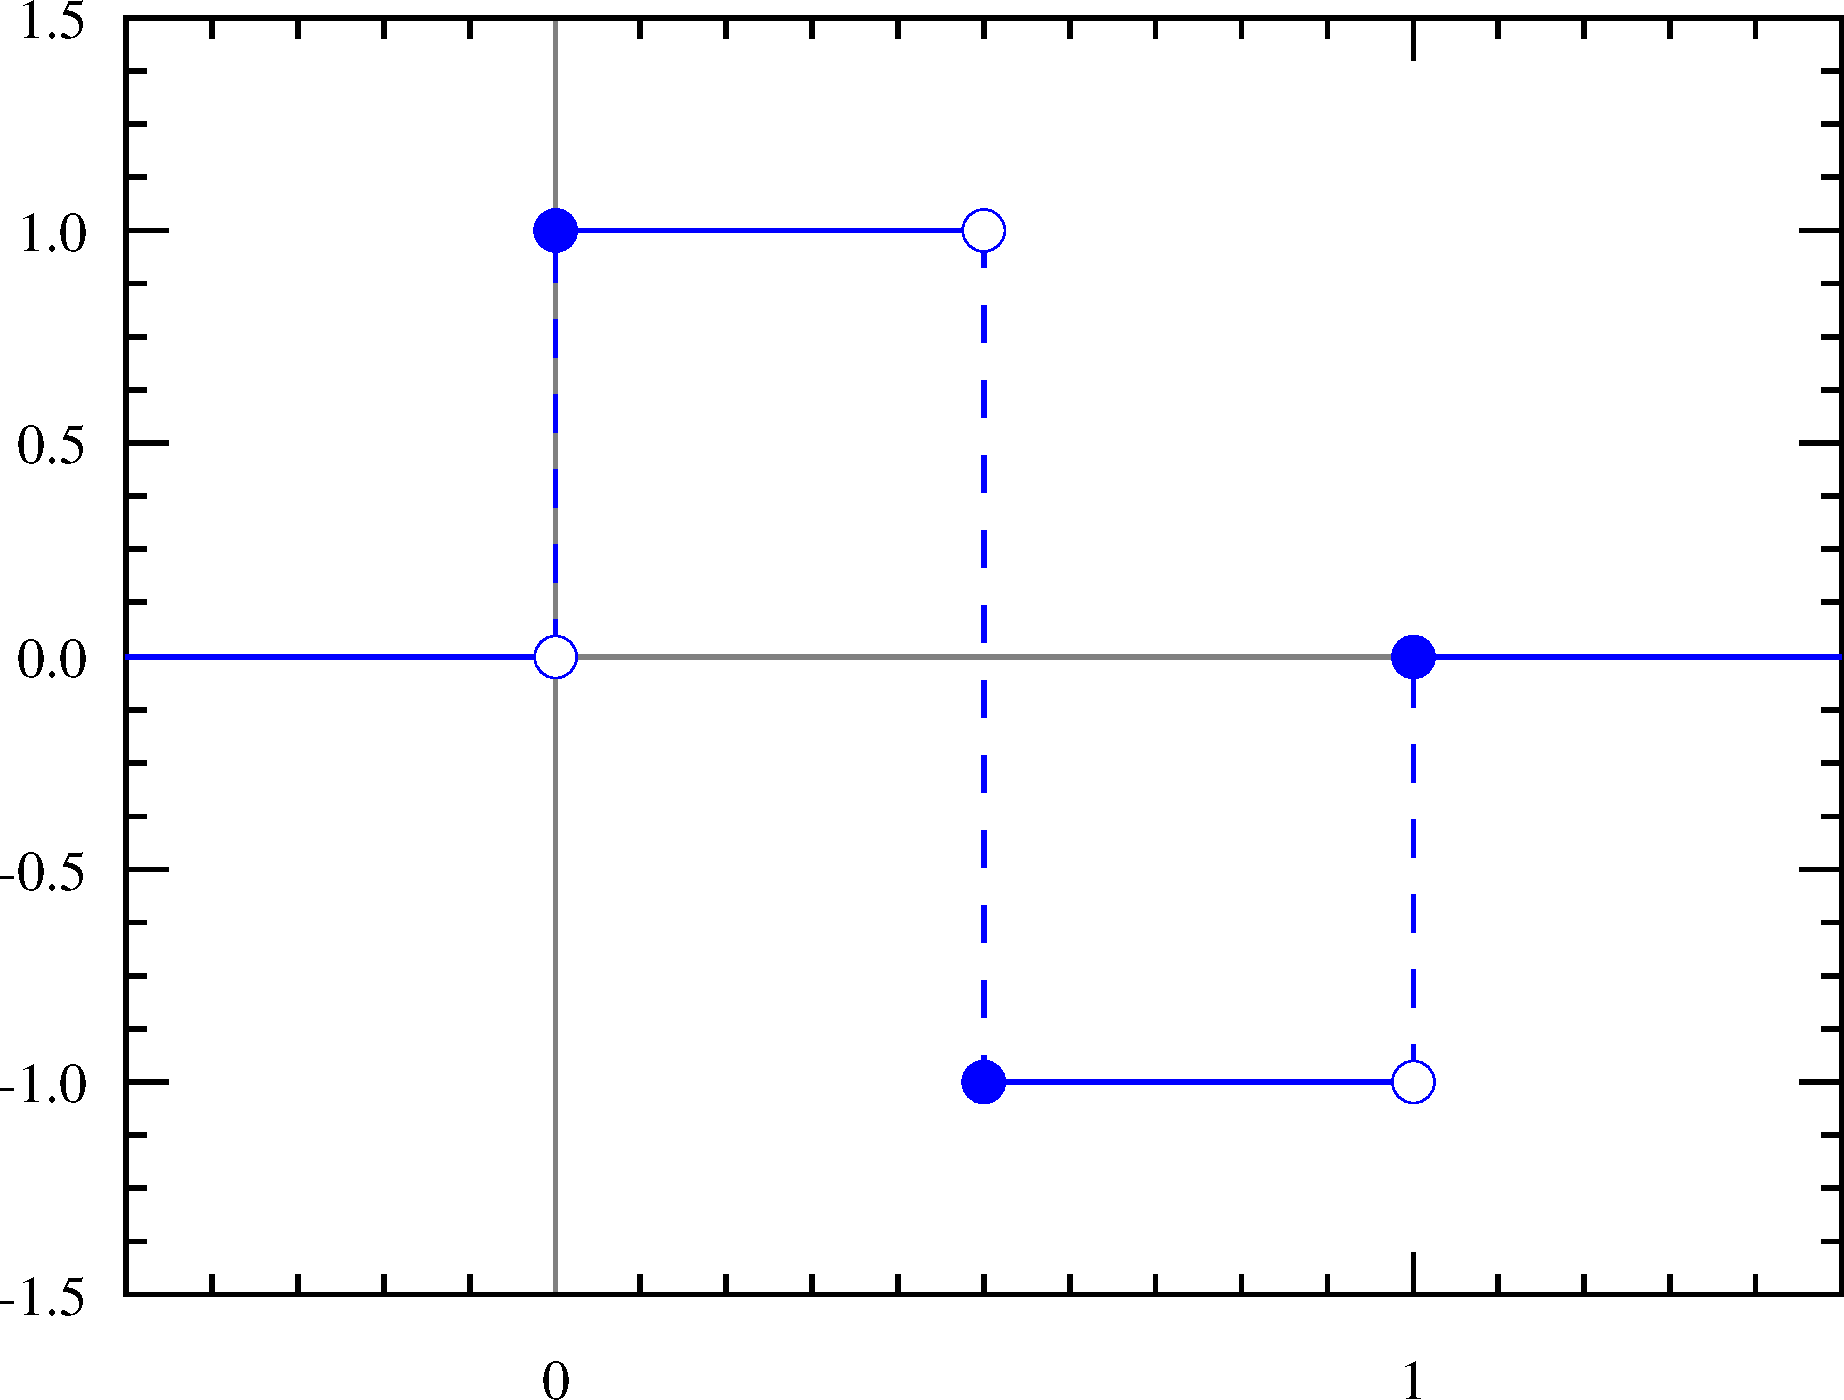
\includegraphics[width=.7\linewidth]{Haar_wavelet.pdf}
 \caption{Haar wavelets. From wikipedia, author Omegatron.}
 \label{fig:wavelets:matlab:haar}
\end{figure}

\subsubsection{Simple 1D decomposition}
\begin{matlab}
function C = simpleWaveDec(signal, nb_scales)
% wavelet decomposition of <signal> into <nb_scales> scales
% This function uses Haar wavelets for demonstration purposes.

% Haar Wavelets filters for decomposition and reconstruction
ld = [1 1];
hd = [-1 1];

% transformation
C=cell(nb_scales+1, 1);
A = signal; % approximation
for i=1:nb_scales
    [A, D] = waveSingleDec(A, ld, hd);
    % get the coefficients
    C{i}=D;
end
C{nb_scales+1}=A;
\end{matlab}

\begin{matlab}
% function single step wavelet decomposition
function [A, D]=waveSingleDec(signal, ld, hd)
% 1D wavelet decomposition into
% A: approximation vector
% D: detail vector
% ld: low pass filter
% hd: high pass filter

% convolution
A = conv(signal, ld, 'same');
D = conv(signal, hd, 'same');

% subsampling
A = A(1:2:end);
D = D(1:2:end);
\end{matlab}

\subsubsection{Simple 1D reconstruction}
The reconstruction starts from the highest scale and computes the approximation signal with the given details.
\begin{matlab}
function A = simpleWaveRec(C)
% wavelet simple reconstruction function of a 1D signal
% C: Wavelet coefficients 
%
% The Haar wavelet is used
ld = [1 1];
hd = [-1 1];
lr = ld/2;
hr = -hd/2;

nb_scales = length(C)-1;
A = C{nb_scales+1};
for i=nb_scales:-1:1
    A = waveSingleRec(A, C{i}, lr, hr);
end
\end{matlab}

\begin{matlab}
function approx = waveSingleRec(a, d, lr, hr)
% 1D wavelet reconstruction at one scale
% a: vector of approximation
% d: vector of details
% lr: low pass filter defined by wavelet
% hr: high pass filter defined by wavelet
%
% This is Mallat algorithm.
% NB: to avoid side effects, the convolution function does not use the 'same' option

approx = zeros(1, length(a)*2);
approx(1:2:end) = a;
approx = conv(approx, lr);

detail = zeros(1, length(a)*2);
detail(1:2:end) = d;
detail = conv(detail, hr);

approx = approx + detail;
approx = approx(1:length(a)*2);
\end{matlab}
\subsubsection{Results}
\begin{mwindow}
>> signal = [4;8;2;3;5;18;19;20];
>> C = simpleWaveDec(signal,3)
C = 
    [4x1 double]
    [2x1 double]
    [       -45]
    [        79]
    
>> for i=1:4, C{i}, end
ans =
    -4
    -1
   -13
    -1

ans =
     7
   -16

ans =
   -45

ans =
    79
\end{mwindow}


\subsection{2D signals}
\subsubsection{Decomposition}
\begin{matlab}
%% 2D simple wavelet decomposition
function [LcLrA, HcLrA, LcHrA, HcHrA] = decWave2D(image, ld, hd)
% wavelet decomposition of a 2D image into four new images.
% The image is supposed to be square, the size of it is a power of 2 in the x and y dimensions.

% We manipulate doubles
image = double(image);

%% Decomposition on rows
sx=size(image, 1);
sy=size(image, 2);

LrA = zeros(sx, sy/2);
HrA = zeros(sx, sy/2);
for i=1:sx
    [A, D]= waveSingleDec(image(i,:), ld, hd);
    LrA(i,:)= A;
    HrA(i,:)= D;
end


%% Decomposition on cols
LcLrA = zeros(sx/2, sy/2);
HcLrA = zeros(sx/2, sy/2);
LcHrA = zeros(sx/2, sy/2);
HcHrA = zeros(sx/2, sy/2);
for j=1:sy/2
    [A, D]= waveSingleDec(LrA(:,j), ld, hd);
    LcLrA(:,j) = A;
    HcLrA(:,j) = D;
    
    [A, D]= waveSingleDec(HrA(:,j), ld, hd);
    LcHrA(:,j) = A;
    HcHrA(:,j) = D;
end

%% Display result
figure();
subplot(2, 2, 1); imshow(LcLrA, []);
subplot(2, 2, 2); imshow(HcLrA, []);
subplot(2, 2, 3); imshow(LcHrA, []);
subplot(2, 2, 4); imshow(HcHrA, []);
\end{matlab}

\begin{matlab}
function C = simpleImageDec(image, nb_scales)
% wavelet decomposition of <image> into <nb_scales> scales
% This function uses Haar wavelets for demonstration purposes.

% Haar Wavelets filters for decomposition and reconstruction
ld = [1 1];
hd = [-1 1];

% transformation
C=cell(nb_scales+1, 1);
A = image; % approximation

coeffs = cell(3,1);
for i=1:nb_scales
    [A, HcLrA, LcHrA, HcHrA] = decWave2D(A, ld, hd);
    coeffs{1} = HcLrA;
    coeffs{2} = LcHrA;
    coeffs{3} = HcHrA;
    % set the coefficients
    C{i}=coeffs;
end
C{nb_scales+1} = A;
\end{matlab}


\subsubsection{2D reconstruction}
\begin{matlab}
%% 2D simple wavelet reconstruction
function A = recWave2D(LcLrA, HcLrA, LcHrA, HcHrA, lr, hr)
% Reconstruction of an image from lr and hr filters and from the wavelet decomposition.
% A: resulting (reconstructed) image
%
% NB: This algorithm supposes the number of pixels in x and y dimensions is
% a power of 2.

[sx, sy] = size(LcLrA);

%% Allocate temporary matrices
LrA = zeros(sx*2, sy);
HrA = zeros(sx*2, sy);
A   = zeros(sx*2, sy*2);

%% Reconstruct from cols
for j=1:sy,
    LrA(:,j) = waveSingleRec(LcLrA(:,j), HcLrA(:,j), lr, hr);
    HrA(:,j) = waveSingleRec(LcHrA(:,j), HcHrA(:,j), lr, hr);
end

%% Reconstruct from rows
for i=1:sx*2,
    A(i,:) = waveSingleRec(LrA(i,:), HrA(i,:), lr, hr);
end

%% Display reconstructed image
figure();
imshow(A,[]);
\end{matlab}

\begin{matlab}
function A = simpleImageRec(C)
% wavelet reconstruction of an image described by the wavelet coefficients C 

% The Haar wavelet is used
ld = [1 1];
hd = [-1 1];
lr = ld/2;
hr = -hd/2;

nb_scales = length(C)-1;
A = C{nb_scales+1};
for i=nb_scales:-1:1
    A = recWave2D(A, C{i}{1}, C{i}{2}, C{i}{3}, lr, hr);
end

\end{matlab}

\subsubsection{Results}
The illustration Fig. \ref{fig:wavelets:matlab:lena_lvl} is obtained by the following code. The useful functions are presented below.
\begin{sh}
>> I = imread('lena256.png')
>> C = simpleImageDec(I, 3);
>> A = displayImageDec(C);
>> imwrite(uint8(255*A), 'lena_3lvl.png');
\end{sh}

\begin{matlab}
function [ A ] = displayImageDec( C )
% Construct a single image from a wavelet decomposition
% C: the decomposition
% A: the entire illustration image

n_scales = length(C)-1;
[n, m] = size(C{1}{1});
A = zeros(2*n, 2*m);

prev = C{n_scales+1};
for s=n_scales:-1:1
    ns = n / 2^(s-2);
    ms = m / 2^(s-2);
    A(1:ns, 1:ms) = imdec2im(prev, C{s});
    prev = A(1:ns, 1:ms);
end

end
\end{matlab}

\begin{matlab}
function A = imdec2im(LcLrA, lvlC)
% constructs a single image from:
% LcLrA: the approximation image
% lvlC: the wavelet decomposition at one level
%
% for display purposes

HcLrA=lvlC{1};
LcHrA=lvlC{2};
HcHrA=lvlC{3};
[n, m] = size(HcLrA);

A = zeros(2*n, 2*m);

% approximation image can be with high values when using Haar coefficients
A(1:n, 1:m) =LcLrA/ max(LcLrA(:));

% details are low, and can be negative
A(1:n, m+1:2*m) = imadjust(HcLrA, stretchlim(HcLrA), [0 1]);
A(n+1:2*n, 1:m) = imadjust(LcHrA, stretchlim(LcHrA), [0 1]);
A(n+1:2*n, m+1:2*m) = imadjust(HcHrA, stretchlim(HcHrA), [0 1]);

imshow(A)
\end{matlab}


\begin{figure}[htbp]
 \centering
 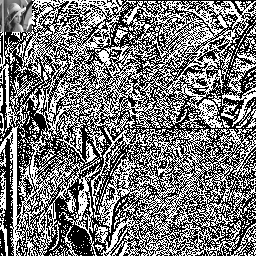
\includegraphics[width=10cm]{lena_3lvl.png}
 \caption{(Haar) Wavelet decomposition of the Lena image.}
 \label{fig:wavelets:matlab:lena_lvl}
\end{figure}


\subsection{Matlab functions}

\subsubsection{1D}
Example on a sample function:
\begin{matlab}
% signal
t=0:.001:10;
signal = sin(2*pi*3*t)+.2*sin(2*pi*50*t);

% parameters
wavelet = 'db1'; % Daubechies wavelets
lvl = 5; % decomposition level

% Decomposition
[C, S] = wavedec(signal, lvl, wavelet);

% Reconstruction
srec = waverec(C, S, wavelet);
\end{matlab}


\subsubsection{2D}
\begin{matlab}
% read an image
I = imread('Couche_18.png');
lvl = 8;

% decomposition
[C, S] = wavedec2(I, lvl, 'db4');

% threshold after lvl
newC = wthcoef2('a', C, S);

% reconstruction
I2 = waverec2(newC, S, 'db4');

% display result
imshow(I,[]);

figure(); imshow(I2,[]);
\end{matlab}
